\documentclass{winnower}
\usepackage{graphicx}
\begin{document}

\title{Learning Convolutional Neural Network Structure}

\author{Christopher Salotti}
\affil{Image Science Laboratory, Technicolor Rennes}
\author{Joaquin Zepeda}
\affil{Image Science Laboratory, Technicolor Rennes}
\author{Patrick Perez}
\affil{Image Science Laboratory, Technicolor Rennes}



\date{}

\maketitle

%\begin{abstract}

%\end{abstract}


\section{Introduction}
Machine learning has long proven its capacity to perform tasks in an efficient way, especially concerning those related to vision and images. It has also proven its inefficiency to process raw data and used instead more convenient representations, such as SIFT or HOG, to perform detection or classification. However, those transformation were manually build and carefully designed and, at some points, limitations started to appear in term of performance and results. Building new transformations is a tough process where engineers tried to think about what kind of features can be useful to extract for a given task.

Deep Learning techniques tackle this problem by performing several non-linear transformations through multiple layers.  
Instead of using a predefined method to directly extract features from images, it learns them by using a general-purpose learning procedure. It results in outstanding improvements in computer vision and state-of-the-art results never achieved before, both in supervised and unsupervised learning. 

Since the first proposed architecture \cite{krizhevsky2012imagenet} that won the famous ImageNet contest, the Convolutional Neural Networks have been greatly improved by adding a large number of layers. However, issues started to arise, such as explosions of the number of parameters or the vanishing gradients and, at some point, a deeper network wouldn't bring any better results. Recent solutions, such as \cite{he2015deep}, observed a great degradation in the results accuracy when more layer where added to a network and presented a solution to construct robust Deep Neural Network. 

By observation, a common remark can be made about all those constructions : None of them justify the number and the size of parameters used or even the succession of layer type. In most cases, choices have been made by trying different parameters and choose the ones that gave best results; or in some cases \cite{szegedy2015going}, those parameters where chosen by \textit{standard} use or \textit{convenience}. It results into huge networks with lots of unoptimized parameters that make computation and design choices justifications harder and it has also been observed that these structures are more prone to overfitting. 

In this work, we aim to optimize our network for supervised learning by reducing the number of parameters while keeping an accuracy close to the state-of-the-art results in image classification. We achieve this by adding a penalization to the number, the size and the shape of convolutional kernels.

\section{Methodology} 
Our work consider the specific use of Convolutional Neural Networks applied to image classification. The network will have to \textit{learn} how to properly \textit{represents} those image and \textit{decide} to which class they belong to.

Let us consider a Convolutional Neural Network $f$ with the parameters  $\theta_1$ that take an image $J \in \mathbb{R}^{h \times w \times c}$ as input and output a feature map $x \in \mathbb{R}^{d}$ after propagating through $L$ layers  : $f(I, \theta_1) = O$. 

We consider only convolutional layer, thus the output of a hidden layer $h_l$ with $N_l$ filters $K^l_i$, with $1 \leq i \leq N_l$, for input feature maps $\textbf{u} \in \mathbb{R}^{h' \times w' \times c'}$ produces output feature maps $\textbf{v} \in \mathbb{R}^{h'' \times w'' \times c''}$: $\textbf{v} = h(K^l, \textbf{x})$. 

Finally, we consider a decision function $g$ with parameters $\theta_2$ that take the output feature map $O$ as an input and decide in which of the $N_c$ classes $c_j$, with $1 \leq j \leq N_c $, the image belongs to : $c_j = g(O,\theta_2)$.

The overall purpose of a Convolutional Neural Network is to learn parameters $\Theta \in \{ \theta_1, \theta_2 \}$ by training a large dataset of labelled images $(J_i, y_i)$, where $y_i$ is the label, and perform the learning by minimizing the task-specific objective :
\[
	\arg\!\min_{\Theta} \dfrac{1}{N} \sum_{i=1}^N l(g(f(J_i, \Theta), y_i) + \lambda R(\Theta) 
\]


Where $l$ is the penalty and $R$ the regularization term. Without going into details about the penalty function, we will focus on our regularization term. Usually, regularization is used to overcome the eternal overfitting problem in machine learning. In our use case, we will use it to optimize and reduce the number of parameters to have a more compact and  efficient network.

\subsection{Kernel cardinality regularization}

As describe above, our convolutional network consists of a succession of layers performing convolutions between kernels $K_i^l$ and input features $u$. Usually, the number of those kernels ($N_l$) is simply a construction choice without any justifications and, since we want a more compact network, we enforce sparsity into those kernels by applying a specific use of the famous \textit{lasso} ($l_1$) penalty called the \textit{group lasso}. We consider all the kernels on each layer and group their respective $l_2$ norm as a regularization term, also called the $L_{2,1}$ norm. Thus, we have our first regularization term :
\[
	R_1(\Theta) = \|K\|_{2,1} = \sum_l \|K^l\|_2 = \sum_l\sqrt{\sum\nolimits_{i = 1}^{N_l} (K_i^l)^2}
\] 

Therefore, we force weights in the kernel to be 0 until some become totally empty such as their impact on the network is nullified.

\subsection{Kernel size regularization }

Similarly to the number of kernels, their size is simply a choice of convenience or standard use without any justifications. Typical sizes used by architecture are odd ones (e.g $3 \times 3$, $5 \times 5$ and $7 \times 7$) and no considerations are done for even ones. Although kernel sizes can change between layers, there isn't any variety in their shape inside a layer. This constraint can be an issue for generalization purpose, but also a restraint in the convergence of the learning procedure.

The solution we propose is also a $l_{2,1}$ regularization on kernel regions. As shown in Figure \ref{fig:kernel-rings}, weights $w_{ij}$ a separated into several pseudo rings $\underline{r}_i$.

\begin{figure}[h!]
\centering
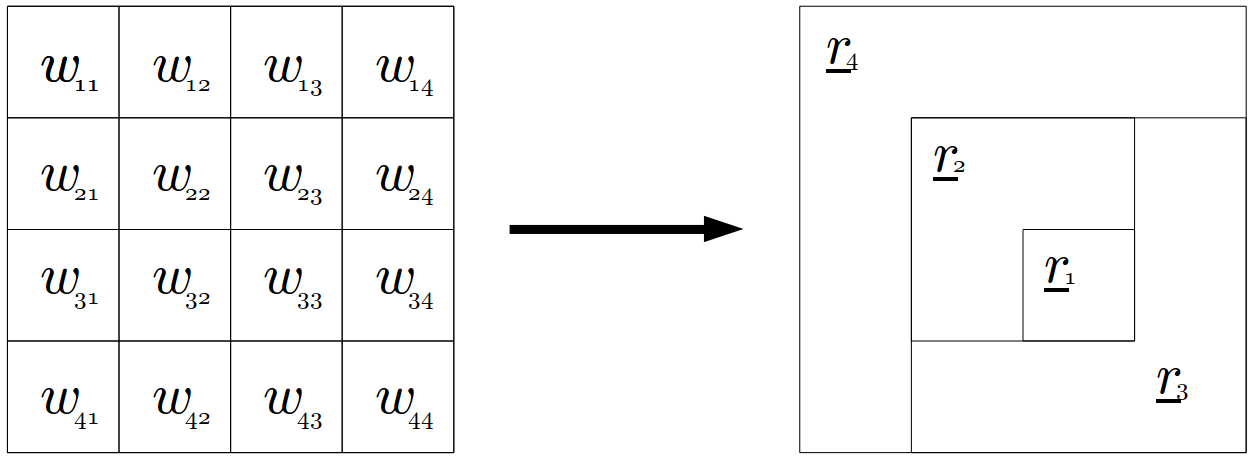
\includegraphics[width=0.7\textwidth]{pic/kernel_split.png}
\caption{Example of a $4 \times 4$ kernel partitionned into $4$ pseudo-rings}
\label{fig:kernel-rings}
\end{figure}

Similar to kernels in our previous regularizations, we try to enforce sparsity in each rings with the following rule : if a ring $r_i$ is empty, thus all the $r_j$ for $j > i$ should also be empty. Therefore, we adopt the following grouping for the $l_{2,1}$ regularization :

\[
G^{ks} =  
\begin{bmatrix}
	\|\underline{r}_4 \|_2 \\
	\|\left[\underline{r}_4^\top, \underline{r}_3^\top \right]^\top \|_2 \\
	\|\left[\underline{r}_4^\top, \underline{r}_3^\top, \underline{r}_2^\top \right]^\top\|_2 \\
	\|\left[\underline{r}_4^\top, \underline{r}_3^\top, \underline{r}_2^\top, \underline{r}_1^\top \right]^\top\|_2
\end{bmatrix}
\]
and the second regularization term for all kernels in every layer become 
\[
R_2(\Theta) = \| G^{ks} \|_1 = \sum_i G^{ks}_i
\]

\subsection{Kernel shape regularization}
We mentioned before that constraints on sizes and shapes could significantly slow down our optimization and some meaningful features properties could be lost. The size regularization approach only consider square kernel, a subclass of all possible convolution filters. Thus, as an alternative approach, we propose a similar region-based regularization to enable a larger pool of possible shapes for kernels. As shown in Figure \ref{fig:kernel-slices}, vectors are sliced in an horizontal and vertical manner. Similar to rings, we try to enforce sparsity by grouping slices in such a way that external ones are sparse before the internal ones. Thus, for the kernel $K$ in figure \ref{fig:kernel-slices} 
\[
	\Omega_H(K) = 
	\begin{bmatrix}
		\|\underline{c}_1 \|_2 \\
		\|\left[\underline{c}_1^\top, \underline{c}_4^\top \right]^\top \|_2 \\
		\|\left[\underline{c}_1^\top, \underline{c}_2^\top, \underline{c}_4^\top \right]^\top\|_2 \\
		\|\left[\underline{c}_1^\top, \underline{c}_2^\top, \underline{c}_3^\top, \underline{c}_4^\top \right]^\top\|_2
	\end{bmatrix},
	\Omega_V(K) = 
	\begin{bmatrix}
		\|\underline{l}_1 \|_2 \\
		\|\left[\underline{l}_1^\top, \underline{l}_4^\top \right]^\top \|_2 \\
		\|\left[\underline{l}_1^\top, \underline{l}_2^\top, \underline{l}_4^\top \right]^\top\|_2 \\
		\|\left[\underline{l}_1^\top, \underline{l}_2^\top, \underline{l}_3^\top, \underline{l}_4^\top \right]^\top\|_2
	\end{bmatrix}
\]  
And our second regularization term become 
\[
	R_2(\Theta) = \|\Omega_H(K)\|_1 + \|\Omega_V(K)\|_1
\]
\begin{figure}[h!]
\centering
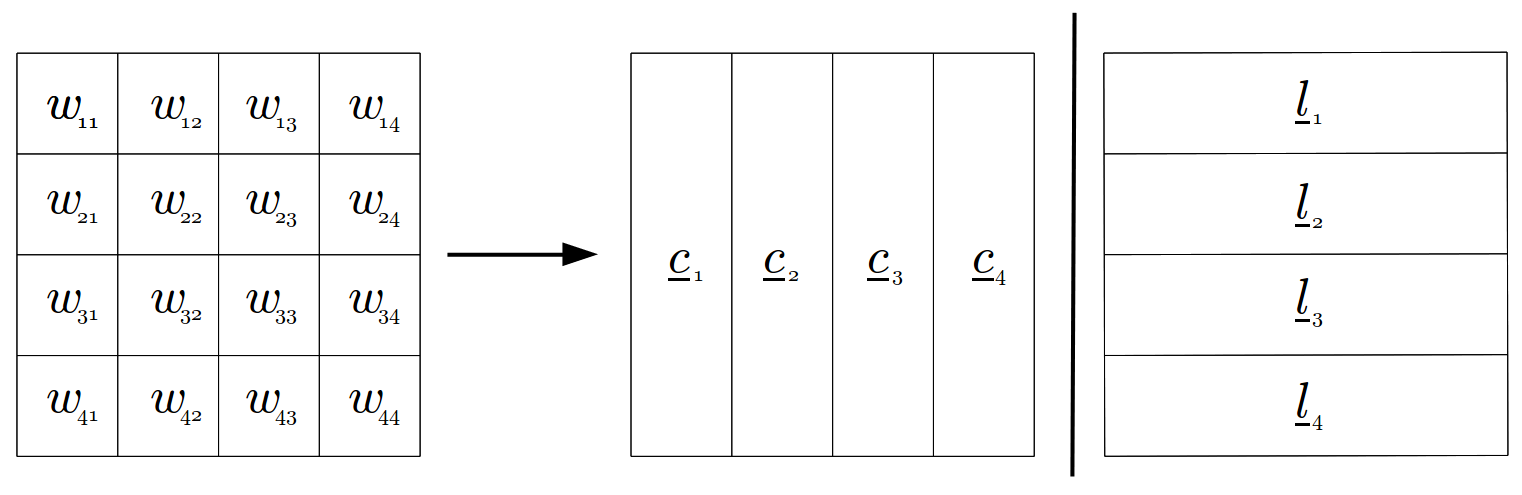
\includegraphics[width=0.9\textwidth]{pic/kernel_col_row.png}
\caption{Example of a $4 \times 4$ kernel with $4$ vertical and horizontal slices}
\label{fig:kernel-slices}
\end{figure}

Implementation details : Since we could end up with kernel of different size in our layer, we could encounter some computational and implementation constraints due to the characteristic of our API Tensorflow. To overcome this problem, we can simply consider only single filters per layer and, since output feature maps will have the same size, simply concatenate the resulting results into a single 3D tensors.

\subsection{Kernel input feature map activations regularization}
Convolution Neural Networks are successions of non-linear transformations performed on layers. In a single layer, input feature maps $u$ is filtered through a collection of $N_l$ kernels that produce output feature maps $v$. However, feature maps are collection of matrices merged together to form a tensor. By performing activations on all feature maps, tensors might do redundant or unnecessary computation. The feature maps regularization would consists of the same spirit behind all our regularizations : Remove activations on specific feature map depth for kernel by enforcing sparsity. Similar to rings and slices, we consider each feature map as a single group for regularization, but we allow activation for a specific feature map to be sparse without any consequences on other ones(In other words, they are independent from each others).

Considering a kernel on layer $l$, $K^l \in \mathbb{R}^{r \times c \times d}$, as a composition of feature map activations matrices, $\{ K^l_i \}_{i=1}^d $ with  $K^l_i \in \mathbb{R}^{r \times c}$, our third regularization term become 
\[
R_3(\Theta) = \|K^l\|_{1,2} = \sum_{i=1}^d \|K_i^l \|_2 
\]



\subsection{Implementations details}
In term of implementations, we decided to try our regularizations on the famous Residual Networks proposed by Microsoft. We will also study the case of non-residual network to see whether their construction have an influence on the optimization of the parameters.

In term of software, Tensorflow is used to build and train every model. We found it really convenient, since Tensorflow is provided with useful monitoring tools, but also benefits from a large community that provided useful tips for further improvements.



\bibliographystyle{abbrv}
\bibliography{cnn_arch}



\end{document}